\ifx\allfiles\undefined
\documentclass[12pt, a4paper, oneside, UTF8]{ctexbook}
\def\path{../config}
\input{\path/package.tex}

% 定理环境设置
\input{\path/theorem1_zh.tex}

\input{\path/custom.tex}

% 修改参数改变封面样式，0 默认原始封面、内置其他1、2、3种封面样式
\def\myIndex{3}


\ifnum\myIndex>0
    \input{\path/cover_package_\myIndex} 
\fi

\def\myTitle{高等数学笔记}
\def\myAuthor{M.K.}
\def\myDateCover{\today}
\def\myDateForeword{\today}
\def\myForeword{前言}
\def\myForewordText{
    
    这是一个基于\LaTeX{}模板的高数笔记．
    内容参考了包括但不限于以下资料：
    \begin{itemize}
        \item 《高等数学》（同济大学出版社）第七版
        \item 《吉米多维奇高等数学习题精选精讲》（山东科学技术出版社）第二版
        \item 《高等数学作业集》（哈尔滨工业大学出版社）第一版
        \item \href{https://space.bilibili.com/1035929235}{B站UP主：一高数}的高数课程
        \item \href{https://space.bilibili.com/42428180}{B站UP主：考研竞赛数学}的试题讲解与高数课程
        \item \href{https://space.bilibili.com/391930545}{B站UP主：Maki的完美算数教室}的高数内容

    \end{itemize}

    封面来源于\href{https://www.pixiv.net/users/3952}{おにねこ}的作品\href{https://www.pixiv.net/artworks/136551599}{雨雫とプレアデス}
    如有侵权请联系我删除．
}
\def\mySubheading{副标题}


\begin{document}
% \input{../config/cover}
\else
\fi
\chapter{一元函数积分学}
\section{积分表节选}
\begin{align*}
\int & \dfrac{1}{1+x^2} \d x = \arctan x + C &
\int & \dfrac{1}{\sqrt{1-x^2}} \d x = \arcsin x + C \\
\int & a^x \d x = \frac{a^x}{\ln a} + C, (a>0, a \neq 1) &
\int & \sec^2 x \d x = \tan x + C \\
\int & \csc^2 x \d x = -\cot x + C &
\int & \sec x \tan x \d x = \sec x + C \\
\int & \csc x \cot x \d x = -\csc x + C &
\int & \sec x \d x = \ln |\sec x + \tan x| + C \\
\int & \csc x \d x = \ln |\csc x - \cot x| + C &
\int & \tan x \d x = -\ln |\cos x| + C \\
\int & \cot x \d x = \ln |\sin x| + C &
\int & \dfrac{\d x}{x^2 + a^2} = \dfrac{1}{a} \arctan \dfrac{x}{a} + C,(a > 0) \\
\int & \dfrac{\d x}{\sqrt{x^2 \pm a^2}} = \ln |x + \sqrt{x^2 \pm a^2}| + C, (a > 0) &
\int & \dfrac{\d x}{\sqrt{a^2 - x^2}} = \arcsin \dfrac{x}{a} + C, (a > 0) \\
\int & \dfrac{\d x}{a^2 - x^2} = \dfrac{1}{2a} \ln \left| \dfrac{a+x}{a - x} \right| + C, (a > 0)
\end{align*}
\section{三角函数积分}
\subsection{配凑法}
\begin{example}
    计算积分$\displaystyle \int \dfrac{\d x}{3 +\sin^2 x}$
\end{example}
\begin{solution}
    \begin{align*}
        \int \dfrac{\d x}{3 +\sin^2 x} &= \int \dfrac{\sec^2 x}{3(1+\tan^2 x) + \tan^2 x}\d x = \int \dfrac{\d \tan x}{3 + 4\tan^2 x} \\
        &=\dfrac{1}{2} \int \dfrac{\d (2\tan x)}{3 + (2\tan x)^2} = \dfrac{1}{2\sqrt{3}} \arctan \dfrac{2\tan x}{\sqrt{3}} + C
    \end{align*}
\end{solution}
\begin{myRemark}
    三角函数积分常用替换方法：
    \begin{itemize}
        \item 若 $\sin x$ 为奇次幂、$\cos x$ 为偶次幂，则利用 $\d \cos x$ 或 $\d \sin x$ 进行替换；
        \item 若 $\cos x$ 为奇次幂、$\sin x$ 为偶次幂，则利用 $\d \sin x$ 或 $\d \cos x$ 进行替换；
        \item 若 $\sin x, \cos x$ 均为偶次幂或均为奇次幂，则利用 $\d \tan x$ 或 $\d \cot x$ 进行替换．
    \end{itemize}
\end{myRemark}
\begin{example}
    计算积分$\displaystyle \int \dfrac{\d x}{\sin^3 x \cdot \cos x}$
\end{example}
\begin{solution}
    \begin{align*}
        \int \dfrac{\d x}{\sin^3 x \cdot \cos x} = \int \dfrac{\sec^4 x}{\tan^3 x} \d x 
        = \int \dfrac{\tan^2 x + 1}{\tan^3 x} \d \tan x
        = \ln |\tan x|-\dfrac{1}{2\tan^2 x} + C
    \end{align*}
\end{solution}
\begin{example}
    计算积分$\displaystyle \int \dfrac{\ln \tan x}{\sin x \cdot \cos x} \d x$
\end{example}
\begin{solution}
    \begin{align*}
        \int \dfrac{\ln \tan x}{\sin x \cdot \cos x} \d x
        =\int \dfrac{\ln \tan x}{\tan x}\d \tan x
        =\int \ln \tan x \,\d (\ln \tan x)
        =\dfrac{1}{2}\ln^2(\tan x)
    \end{align*}
\end{solution}
\begin{example}
    计算积分$\displaystyle \int \tan^3 x \sec x \d x$
\end{example}
\begin{solution}
    \begin{align*}
        \int \tan^3 x \sec x \d x
        =\int \tan^2 x \d \sec x
        =\int (\sec^2 x -1) \d \sec x
        =\dfrac{1}{3}\sec^3 x - \sec x + C
    \end{align*}
\end{solution}
\begin{example}
    计算积分$\displaystyle\int \tan^4 x \d x$
\end{example}
\begin{solution}
    \begin{align*}
        \int \tan^4 x \d x
        &=\int \tan^2 (\sec^2 -1)\d x
        =\int \tan^2 \d \tan x-\int \sec^2 -1\;\d x\\
        &=\dfrac{1}{3}\tan^3 x-\tan x+x +C
    \end{align*}
\end{solution}
\begin{example}
    计算积分$\displaystyle \int \dfrac{1}{\sin^3 x} \d x$
\end{example}
\begin{solution}
    \begin{align*}
        \int \dfrac{1}{\sin^3 x} \d x
        &=-\int \csc x\,\d \cot x = -\csc x\cot x + \int \cot x \d \csc x\\
        &=-\csc x\cot x - \int \csc x \cot^2 x \d x\\
        &=-\csc x\cot x - \int \csc x (\csc^2 x - 1) \d x\\
        &=-\csc x\cot x - \int \dfrac{1}{\sin^3 x} \d x + \ln |\csc x - \cot x|
    \end{align*}
    移项化简得
    \[
        \int \dfrac{1}{\sin^3 x} \d x = \dfrac{1}{2} \left( \ln |\csc x - \cot x| -\csc x\cot x \right) + C
    \]
\end{solution}
\subsection{一次分母三角分式的处理}
\begin{example}
    计算积分$\displaystyle \int \frac{3\cos x-\sin x}{\cos x-2\sin x}$
\end{example}
\begin{solution}
    \begin{align*}
        \int \dfrac{3\cos x - \sin x}{\cos x - 2\sin x} \d x
        &= \int \dfrac{(\cos x -2\sin x)-(-\sin x-2\cos x)}{\cos x - 2\sin x} \d x\\
        &= \int 1 - \dfrac{\d (\cos x-2\sin x)}{\cos x - 2\sin x}\\
        &= x + \ln |\cos x - 2\sin x| + C
    \end{align*}
\end{solution}
\begin{myRemark}
    对于形如$\displaystyle \int \dfrac{A\sin x + B\cos x}{C\sin x + D\cos x} \d x$的积分，
    可将分子配凑成分母的常数倍加上分母的导数倍，从而将积分化为易积的形式．
\end{myRemark}
\begin{example}
    计算积分$\displaystyle \int \dfrac{1}{\sin x+\cos x} \d x$
\end{example}
\begin{solution}
    $\displaystyle\int \dfrac{1}{\sin x+\cos x} \d x
    =\dfrac{1}{\sqrt{2}}\int \frac{\d (x + \frac{\pi}{4})}{\sin (x + \frac{\pi}{4})}
    =\dfrac{1}{\sqrt{2}} \ln \left| \csc (x + \frac{\pi}{4}) - \cot (x + \frac{\pi}{4}) \right| + C$
\end{solution}
\begin{myRemark}
    对于形如$\displaystyle \int \dfrac{1}{a\sin x + b\cos x} \d x$的积分，
    可将分母化为单一三角函数形式，从而将积分化为易积的形式．
\end{myRemark}
\subsection{万能代换}
\begin{theorem}
    设$f(\sin x, \cos x)$在区间$I$上连续，则在$I$上有
    \[
        \int f(\sin x, \cos x) \d x = \int f\left( \dfrac{2u}{1+u^2}, \dfrac{1-u^2}{1+u^2} \right) \cdot \dfrac{2}{1+u^2} \d u
    \]
    其中$u=\tan \dfrac{x}{2}$
\end{theorem}
\begin{example}
    计算积分$\displaystyle\int \dfrac{\d x}{1+\sin x + \cos x}$
\end{example}
\begin{solution}
    \begin{align*}
        \int \dfrac{\d x}{1+\sin x + \cos x}
        &\xlongequal{u=\tan \dfrac{x}{2}}\int \dfrac{\frac{2}{1+u^2}}{1+\frac{2u}{1+u^2}+\frac{1-u^2}{1+u^2}}\d u
        =\int \dfrac{\d u}{1+u}
        =\ln |1+u|+C\\[6pt]
        &=\ln \left|\tan \dfrac{x}{2}+1\right|+C
    \end{align*}
\end{solution}
\begin{example}
    计算积分$\displaystyle\int \dfrac{\d x}{1+\sin x}$
\end{example}
\begin{solution}
    法一:
    \begin{align*}
        \int \dfrac{\d x}{1+\sin x}
        &\xlongequal{u=\tan \dfrac{x}{2}}\int \dfrac{2}{1+u+u^2}\d u
        =2\int \dfrac{1}{(1+u)^2}\d (1+u)
        =\dfrac{-2}{1+u}+C\\
        &=-\dfrac{2}{1+\tan \frac{x}{2}}+C
    \end{align*}
    法二：
    \begin{align*}
        \int \dfrac{\d x}{1+\sin x}
        =\int \dfrac{1-\sin x}{(1+\sin x)(1-\sin x)}\d x
        =\int \dfrac{\d x}{\cos^2 x}-\int \dfrac{\sin x}{\cos^2 x}\d x
        =\tan x - \dfrac{1}{\cos x}+C
    \end{align*}
\end{solution}
\section{反常积分}
\subsection{反常积分敛散性}
\begin{theorem}[常用反常积分敛散性结论]
    设$p,q \in \R$，则有以下结论：
    \begin{enumerate}
        \item 无穷限反常积分 $\displaystyle\int_{a}^{+\infty} \dfrac{1}{x^p\ln^q x} \d x$ ($a>1$) 的敛散性：
        \[
            \begin{cases}
                \text{收敛}, & p>1 \text{ 或 } p=1, q>1 \\
                \text{发散}, & p<1 \text{ 或 } p=1, q \le 1
            \end{cases}
        \]
        \item 瑕积分 $\displaystyle\int_{0}^{a} \dfrac{1}{x^p\ln^q x} \d x$ ($0<a<1$) 的敛散性：
        \[
            \begin{cases}
                \text{收敛}, & p<1 \text{ 或 } p=1, q>1 \\
                \text{发散}, & p>1 \text{ 或 } p=1, q \le 1
            \end{cases}
        \]
        \item 瑕积分 $\displaystyle\int_{a}^{b} \dfrac{1}{(x-a)^p (b-x)^q} \d x$ 的敛散性：
        \[
            \begin{cases}
                \text{收敛}, & p<1, q<1 \\
                \text{发散}, & p \ge 1 \text{ 或 } q \ge 1
            \end{cases}
        \]
    \end{enumerate}
\end{theorem}
\begin{theorem}
设 $f,g$ 为定义在区间 $I$ 上的函数（考虑相应的反常积分），$I_1,I_2\subseteq I$，则：
\begin{enumerate}
    \item 若 $\displaystyle\int_{I_1} f$ 与 $\displaystyle\int_{I_2} g$ 均收敛，则 $\displaystyle\int_I (f+g)$ 收敛；
    \item 若 $\displaystyle\int_{I_1} f$ 收敛而 $\displaystyle\int_{I_2} g$ 发散，则 $\displaystyle\int_I (f+g)$ 发散；
    \item 若 $\displaystyle\int_I f$ 与 $\displaystyle\int_I g$ 均发散，则 $\displaystyle\int_I (f+g)$ 不一定发散（情况不确定）；
    \item 若 $I_1 \cap I_2 = \varnothing$，$\displaystyle\int_{I_1} f$ 在区间 $I_1$ 发散、$\displaystyle\int_{I_2} g$ 在区间 $I_2$ 发散，则 $\displaystyle\int_{I_1}f+\int_{I_2} g$ 发散．
\end{enumerate}
\end{theorem}
\begin{theorem}
    $\forall p \in \R,\displaystyle\int_{0}^{+\infty}\dfrac{\d x}{x^p}$发散
\end{theorem}
\begin{proof}
    \[
        \int_{0}^{+\infty} \dfrac{\d x}{x^p}
        =\int_{0}^{1} \dfrac{\d x}{x^p} + \int_{1}^{+\infty} \dfrac{\d x}{x^p}
    \]
    若原积分收敛，则两个积分均收敛．由已知结论可得$p>1$且$p \le 1$，矛盾，故原积分发散．
\end{proof}
\subsection{反常积分的计算}
\begin{example}
    计算积分$\displaystyle\int_{0}^{\frac{3\pi}{4}} \dfrac{\d x}{1 + \sin^2 x}$
\end{example}
\begin{solution}
    \begin{align*}
        \int_{0}^{\frac{3\pi}{4}} \dfrac{\d x}{1 + \sin^2 x}
        &=\int_{0}^{\frac{3\pi}{4}} \dfrac{\d \tan x}{1 + 2\tan^2 x}
        =\int_{0}^{\frac{\pi}{2}} \dfrac{\d \tan x}{1 + 2\tan^2 x} + \int_{\frac{\pi}{2}}^{\frac{3\pi}{4}} \dfrac{\d \tan x}{1 + 2\tan^2 x}\\
        &=\dfrac{1}{\sqrt{2}} \arctan (\sqrt{2} \tan x) \Bigg|_{0}^{\frac{\pi}{2}} + \dfrac{1}{\sqrt{2}} \arctan (\sqrt{2} \tan x) \Bigg|_{\frac{\pi}{2}}^{\frac{3\pi}{4}}\\
        &=\dfrac{\pi}{\sqrt{2}} + \dfrac{1}{\sqrt{2}}\arctan (-\sqrt{2})
        =\dfrac{\pi}{\sqrt{2}} - \dfrac{1}{\sqrt{2}} \arctan (\sqrt{2})
    \end{align*}
\end{solution}
\begin{myRemark}
    反常积分计算时，若被积函数在区间内有间断点，则需将积分区间依间断点分割成若干部分，
    并对每一部分分别计算反常积分，再将各部分积分结果相加．
\end{myRemark}
\section{定积分的应用}
\subsection{旋转体的体积}
\begin{theorem}
    设平面区域 $D$ 位于直线 $L: Ax+By+C=0$ 的一侧（即 $D$ 与 $L$ 不相交），则区域 $D$ 绕直线 $L$ 旋转一周所形成的旋转体体积 $V$ 为
    \[
        V = \dfrac{2\pi}{\sqrt{A^2 + B^2}} \iint_{D} |Ax + By + C| \d x\d y
    \]
\end{theorem}
\begin{corollary}
    设 $f(x)$ 在 $[a, b]$ 上连续且 $f(x) \ge 0$．由曲线 $y=f(x)$，直线 $x=a, x=b$ ($a<b$) 及 $x$ 轴围成的曲边梯形 $D$：
    \begin{enumerate}
        \item 绕 $x$ 轴旋转一周所得旋转体的体积为
        \[
            V_x = \pi \int_{a}^{b} [f(x)]^2 \d x
        \]
        \begin{center}
            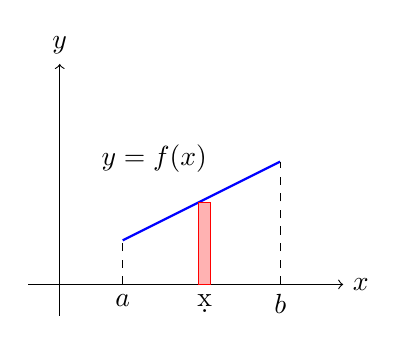
\begin{tikzpicture}[scale=0.8]
                \draw[->] (-0.5,0) -- (4.5,0) node[right] {$x$};
                \draw[->] (0,-0.5) -- (0,3.5) node[above] {$y$};
                \draw[thick, domain=1:3.5, smooth, variable=\x, blue] plot ({\x}, {0.5*\x+0.2});
                \draw[dashed] (1,0) -- (1,0.7);
                \draw[dashed] (3.5,0) -- (3.5,1.95);
                \node[below] at (1,0) {$a$};
                \node[below] at (3.5,0) {$b$};
                \node at (1.5, 2) {$y=f(x)$};
                
                % Volume element (Strip)
                \def\xi{2.2}
                \def\dxi{0.2}
                \def\yi{1.3}
                \fill[red!30] (\xi,0) rectangle (\xi+\dxi, \yi);
                \draw[red] (\xi,0) rectangle (\xi+\dxi, \yi);
                \node[below] at (\xi+0.1, 0) {$\d x$};
            \end{tikzpicture}
        \end{center}
        \item 绕 $y$ 轴旋转一周所得旋转体的体积为
        \[
            V_y = 2\pi \int_{a}^{b} x f(x) \d x \quad (0 \le a < b)
        \]
        \begin{center}
            \begin{tikzpicture}[scale=0.8]
                \draw[->] (-0.5,0) -- (4.5,0) node[right] {$x$};
                \draw[->] (0,-0.5) -- (0,3.5) node[above] {$y$};
                
                % Region
                \draw[thick, domain=1:2.5, smooth, variable=\x, blue] plot ({\x}, {-((\x-1.75)^2)+3});
                \draw[dashed] (1,0) -- (1,2.43);
                \draw[dashed] (2.5,0) -- (2.5,2.43);
                \node[below] at (1,0) {$a$};
                \node[below] at (2.5,0) {$b$};
                
                % Volume element (Strip)
                \def\xi{1.8}
                \def\dxi{0.15}
                \def\yi{2.99}
                \fill[red!30] (\xi,0) rectangle (\xi+\dxi, \yi);
                \draw[red] (\xi,0) rectangle (\xi+\dxi, \yi);
                \node[below] at (\xi+0.075, 0) {$\d x$};
                
                \node at (3.5, 2.5) {柱壳法};
            \end{tikzpicture}
        \end{center}
    \end{enumerate}
\end{corollary}
\begin{myRemark}
    画图是解决旋转体体积问题的关键
\end{myRemark}
\begin{corollary}[极坐标下旋转体体积公式]
    设曲线由极坐标方程 $r=r(\theta)$ ($\alpha \le \theta \le \beta$) 给出．
    \begin{enumerate}
        \item 若 $0 \le \alpha < \beta \le \pi$，则由该曲线与两射线 $\theta=\alpha, \theta=\beta$ 所围成的曲边扇形绕极轴旋转一周所得旋转体的体积为
        \[
            V = \dfrac{2}{3}\pi \int_{\alpha}^{\beta} r^3(\theta) \sin \theta \d \theta
        \]
        \item 若 $-\dfrac{\pi}{2} \le \alpha < \beta \le \dfrac{\pi}{2}$，则由该曲线与两射线 $\theta=\alpha, \theta=\beta$ 所围成的曲边扇形绕垂直于极轴的直线（即 $\theta=\frac{\pi}{2}$）旋转一周所得旋转体的体积为
        \[
            V = \dfrac{2}{3}\pi \int_{\alpha}^{\beta} r^3(\theta) \cos \theta \d \theta
        \]
    \end{enumerate}
    \begin{myRemark}
        限定角度范围是为了保证 $r(\theta) \sin \theta \ge 0$ 以及 $r(\theta) \cos \theta \ge 0$\\
        运用时请务必保证$\cos \theta ,\sin \theta$非负，否则需分段计算（绝对值）
    \end{myRemark}
\end{corollary}
\begin{example}
    计算由曲线$x^2+(y-2a)^2=a^2\;(a>0)$围成的平面图形绕$x$轴旋转一周所得旋转体的体积．
\end{example}
\begin{solution}
    法一：
    由方程$x^2+(y-2a)^2=a^2$可得$y = 2a \pm \sqrt{a^2-x^2}$．
    旋转体体积为
    \begin{align*}
        V &= \pi \int_{-a}^{a} \left[ \left( 2a + \sqrt{a^2-x^2} \right)^2 - \left( 2a - \sqrt{a^2-x^2} \right)^2 \right] \d x \\
        &= \pi \int_{-a}^{a} 8a\sqrt{a^2-x^2} \d x
        = 8\pi a \cdot \dfrac{1}{2}\pi a^2 = 4\pi^2 a^3
    \end{align*}
    法二（柱壳法）：
    选取积分变量为$y$，则$y \in [a, 3a]$．
    旋转体体积为
    \begin{align*}
        V &= \int_{a}^{3a} 2\pi y \cdot 2\sqrt{a^2-(y-2a)^2} \d y
        \xlongequal{y-2a=a\sin t} 4\pi \int_{-\frac{\pi}{2}}^{\frac{\pi}{2}} (2a+a\sin t) \cdot a\cos t \cdot a\cos t \d t \\
        &= 4\pi a^3 \int_{-\frac{\pi}{2}}^{\frac{\pi}{2}} (2\cos^2 t + \sin t \cos^2 t) \d t \\
        &= 4\pi a^3 \left( 2 \cdot \frac{\pi}{2} + 0 \right) = 4\pi^2 a^3
    \end{align*}
\end{solution}
\subsection{旋转体的表面积}
\begin{theorem}
    设平面光滑曲线弧 $L$ 位于直线 $l: Ax+By+C=0$ 的一侧（即 $L$ 与 $l$ 不相交），则 $L$ 绕直线 $l$ 旋转一周所得旋转曲面的面积 $S$ 为
    \[
        S = \dfrac{2\pi}{\sqrt{A^2 + B^2}} \int_{L} |Ax + By + C| \d s
    \]
    其中 $\d s$ 为弧长元素．
\end{theorem}
\begin{corollary}
    设曲线弧 $L$ 由方程 $y=f(x)$ ($a \le x \le b$) 给出，其中 $f(x)$ 在 $[a, b]$ 上有一阶连续导数．
    \begin{enumerate}
        \item $L$ 绕 $x$ 轴旋转一周所得旋转曲面的面积为
        \[
            S = 2\pi \int_{a}^{b} |f(x)| \sqrt{1+[f'(x)]^2} \d x
        \]
        \item $L$ 绕 $y$ 轴旋转一周所得旋转曲面的面积为
        \[
            S = 2\pi \int_{a}^{b} |x| \sqrt{1+[f'(x)]^2} \d x
        \]
    \end{enumerate}
\end{corollary}
\begin{theorem}[参数方程形式]
    设曲线弧 $L$ 由参数方程 $\begin{cases} x=x(t) \\ y=y(t) \end{cases}$ ($\alpha \le t \le \beta$) 给出，其中 $x(t), y(t)$ 在 $[\alpha, \beta]$ 上有一阶连续导数．
    \begin{enumerate}
        \item $L$ 绕 $x$ 轴旋转一周所得旋转曲面的面积为
        \[
            S = 2\pi \int_{\alpha}^{\beta} |y(t)| \sqrt{[x'(t)]^2+[y'(t)]^2} \d t
        \]
        \item $L$ 绕 $y$ 轴旋转一周所得旋转曲面的面积为
        \[
            S = 2\pi \int_{\alpha}^{\beta} |x(t)| \sqrt{[x'(t)]^2+[y'(t)]^2} \d t
        \]
    \end{enumerate}
\end{theorem}
\begin{theorem}[极坐标形式]
    设曲线弧 $L$ 由极坐标方程 $r=r(\theta)$ ($\alpha \le \theta \le \beta$) 给出，其中 $r(\theta)$ 在 $[\alpha, \beta]$ 上有一阶连续导数．
    \begin{enumerate}
        \item $L$ 绕极轴旋转一周所得旋转曲面的面积为
        \[
            S = 2\pi \int_{\alpha}^{\beta} r(\theta)\sin\theta \sqrt{r^2(\theta)+[r'(\theta)]^2} \d \theta
        \]
        \item $L$ 绕垂直于极轴的直线（即 $\theta=\frac{\pi}{2}$）旋转一周所得旋转曲面的面积为
        \[
            S = 2\pi \int_{\alpha}^{\beta} r(\theta)\cos\theta \sqrt{r^2(\theta)+[r'(\theta)]^2} \d \theta
        \]
    \end{enumerate}
\end{theorem}
\begin{example}
    计算星形线 $x^{\frac{2}{3}} + y^{\frac{2}{3}} = a^{\frac{2}{3}}\;(a>0)$ 绕 $x$ 轴旋转一周所得旋转曲面的面积．
\end{example}
\begin{solution}
    星形线的参数方程为 $\begin{cases} x=a\cos^3 t \\ y=a\sin^3 t \end{cases} (0 \le t \le 2\pi)$．
    由对称性，只需求第一象限部分 ($0 \le t \le \frac{\pi}{2}$) 绕 $x$ 轴旋转所得面积的两倍．
    \begin{align*}
        x'(t) &= -3a\cos^2 t \sin t \\
        y'(t) &= 3a\sin^2 t \cos t \\
        \d s &= \sqrt{[x'(t)]^2+[y'(t)]^2} \d t = 3a |\sin t \cos t| \d t
    \end{align*}
    在 $t \in [0, \frac{\pi}{2}]$ 上，$\d s = 3a \sin t \cos t \d t$．
    \begin{align*}
        S &= 2 \cdot 2\pi \int_{0}^{\frac{\pi}{2}} y(t) \d s \\
        &= 4\pi \int_{0}^{\frac{\pi}{2}} a\sin^3 t \cdot 3a \sin t \cos t \d t \\
        &= 12\pi a^2 \int_{0}^{\frac{\pi}{2}} \sin^4 t \d (\sin t) \\
        &= 12\pi a^2 \cdot \dfrac{1}{5} \sin^5 t \Bigg|_{0}^{\frac{\pi}{2}} = \dfrac{12}{5}\pi a^2
    \end{align*}
\end{solution}

\section{积分练习}
\begin{exercise}
    设$I_n = n\displaystyle\int_{1}^{a}\dfrac{\d x}{1+x^n}$，
    其中$a>1$，求$\lim\limits_{x \to \infty}I_n$.
\end{exercise}
\begin{solution}
    记$b=\dfrac{1}{a}$，令$t=\dfrac{1}{x}$，则$0<b<1$，有
    \begin{align*}
        I_n &= \int_{b}^{1} \dfrac{nt^{n-1}}{t(1+t^n)} \d t
        =\int_{b}^{1} \dfrac{1}{t}\d (\ln(1+t^n))
        =\left.\dfrac{\ln(1+t^n)}{t}\right|_{b}^{1}+\int_{b}^{1} \dfrac{\ln(1+t^n)}{t^2} \d t\\
        &=\ln 2 - \dfrac{\ln(1+b^n)}{b} + \int_{b}^{1} \dfrac{\ln(1+t^n)}{t^2} \d t
    \end{align*}
    $t \in [b,1]$时，$\dfrac{\ln(1+t^n)}{t^2} \le \dfrac{t^n}{t^2} = t^{n-2}$，故
    \[
        0 \le \int_{b}^{1}\dfrac{\ln(1+t^n)}{t^2} \d t \le \int_{b}^{1} t^{n-2} \d t = \dfrac{1-b^{n-1}}{n-1} \to 0\quad (n \to \infty)
    \]
    而其中显然有$\lim\limits_{n \to \infty} \dfrac{\ln(1+b^n)}{b} = 0$，于是
    \[
        \lim_{n \to \infty} I_n = \ln 2
    \]
\end{solution}
\begin{exercise}
    已知$\displaystyle\int_{0}^{+\infty} \dfrac{\sin x}{x}= \frac{\pi}{2}$，求$\displaystyle\int_{0}^{+\infty} \dfrac{\sin^2 x}{x^2} \d x$.
\end{exercise}
\begin{solution}
    \begin{align*}
        \int_{0}^{+\infty} \dfrac{\sin^2 x}{x^2} \d x
        &=\int_{0}^{+\infty} -\sin^2 x \d \left( \dfrac{1}{x} \right)
        =\left. -\dfrac{\sin^2 x}{x} \right|_{0}^{+\infty} + \int_{0}^{+\infty} \dfrac{2\sin x \cos x}{x} \d x\\
        &=\int_{0}^{+\infty} \dfrac{\sin 2x}{x} \d x
        \xlongequal{t=2x} \int_{0}^{+\infty} \dfrac{\sin t}{t} \d t = \dfrac{\pi}{2}
    \end{align*}
\end{solution}
\begin{exercise}
    试证$\displaystyle\int_{0}^{+\infty} \dfrac{\d x}{1+x^4} = \displaystyle\int_{0}^{+\infty} \dfrac{x^2}{1+x^4} \d x$，并求其值.
\end{exercise}
\begin{proof}
    \[
        \int_{0}^{+\infty} \dfrac{\d x}{1+x^4}
        \xlongequal{t = \frac{1}{x}}\int_{0}^{+\infty} \dfrac{t^2}{1+t^4} \d t
        =\int_{0}^{+\infty} \dfrac{x^2}{1+x^4} \d x
    \]  
    因此
    \begin{align*}
        \int_{0}^{+\infty} \dfrac{\d x}{1+x^4}
        &= \dfrac{1}{2} \int_{0}^{+\infty} \dfrac{1+x^2}{1+x^4} \d x
        =\dfrac{1}{2} \int_{0}^{+\infty} \dfrac{\d \left(x - \dfrac{1}{x}\right)}{\left(x - \dfrac{1}{x}\right)^2 + 2}
        =\dfrac{1}{2\sqrt{2}} \arctan \dfrac{x - \dfrac{1}{x}}{\sqrt{2}} \Bigg|_{0}^{+\infty}\\
        &=\dfrac{\pi}{2\sqrt{2}}
    \end{align*}
\end{proof}
\begin{exercise}
    求$\displaystyle\lim_{n \to \infty} \left( \dfrac{\sin \frac{\pi}{n}}{n+1} + \dfrac{\sin \frac{2\pi}{n}}{n+\frac{1}{2}} + \cdots + \dfrac{\sin \frac{n\pi}{n}}{n+\frac{1}{n}} \right)$.
\end{exercise}
\begin{solution}
    \[
        \lim_{n \to \infty} \sum_{k=1}^{n} \dfrac{\sin \frac{k\pi}{n}}{n + \frac{1}{k}}
        < \lim_{n \to \infty} \frac{1}{n}\sum_{k=1}^{n} \sin \frac{k\pi}{n}
        = \int_{0}^{1} \sin (\pi x) \d x = \dfrac{2}{\pi}
    \]
    \[
        \lim_{n \to \infty} \sum_{k=1}^{n} \dfrac{\sin \frac{k\pi}{n}}{n + \frac{1}{k}}
        > \lim_{n \to \infty} \dfrac{1}{n+1} \sum_{k=1}^{n} \sin \frac{k\pi}{n}
        = \lim_{n \to \infty} \dfrac{n}{n+1} \cdot \dfrac{1}{n} \sum_{k=1}^{n} \sin \frac{k\pi}{n}
        = \int_{0}^{1} \sin (\pi x) \d x = \dfrac{2}{\pi}
    \]  
    故由夹逼定理可得
    \[
        \lim_{n \to \infty} \left( \dfrac{\sin \frac{\pi}{n}}{n+1} + \dfrac{\sin \frac{2\pi}{n}}{n+\frac{1}{2}} + \cdots + \dfrac{\sin \frac{n\pi}{n}}{n+\frac{1}{n}} \right) = \dfrac{2}{\pi}
    \]
\end{solution}
\begin{exercise}
    设定义域为$(0, +\infty)$的连续函数$f(x)$满足$f(xy)=f(x)+f(y)$，试证：$I=\displaystyle\int_{0}^{1} \dfrac{f(1+x)}{1+x^2} \d x = \dfrac{\pi}{8} f(2)$.
\end{exercise}
\begin{proof}
    令$x = y = 1 \Rightarrow f(1) = 0,$令$y = \dfrac{1}{x} \Rightarrow f\left(\dfrac{1}{x}\right) = -f(x)$，则
    \begin{align*}
        I &= \int_{0}^{1} \dfrac{f(1+x)}{1+x^2} \d x
        \xlongequal{x = \tan \theta} \int_{0}^{\frac{\pi}{4}} f(1+\tan \theta) \d \theta
        \xlongequal{ \theta = \frac{\pi}{4} - t} \int_{0}^{\frac{\pi}{4}} f\left(1+\dfrac{1-\tan t}{1+\tan t}\right) \d t\\[6pt]
        &= \int_{0}^{\frac{\pi}{4}} f\left(\dfrac{2}{1+\tan t}\right) \d t
        = \int_{0}^{\frac{\pi}{4}} \left[ f(2) + f\left(\dfrac{1}{1+\tan t}\right) \right] \d t\\[6pt]
        &= \dfrac{\pi}{4} f(2) - \int_{0}^{\frac{\pi}{4}} f(1+\tan t) \d t
        = \dfrac{\pi}{4} f(2) - I
    \end{align*}
    因此$I = \dfrac{\pi}{8} f(2)$.
\end{proof}
\begin{exercise}
    计算积分$\displaystyle\int \frac{e^x (1+\sin x)}{1 + \cos x} \d x$
\end{exercise}
\begin{solution}
    $\displaystyle\int \frac{e^x (1+\sin x)}{1 + \cos x} \d x
    =\displaystyle\int \frac{e^x + e^x \cdot 2\cos \frac{x}{2}\sin \frac{x}{2}}{2\cos^2\frac{x}{2}} \d x
    =\displaystyle\int \frac{e^x + e^x \cdot 2\cos \frac{x}{2}\sin \frac{x}{2}}{2\cos^2\frac{x}{2}} \d x$\\[6pt]
    $\text{\qquad}=\displaystyle\int \left(e^x\cdot\frac{1}{2}\sec^2\frac{x}{2}+e^x\tan\frac{x}{2}\right) \d x
    =\displaystyle\int \d \left(e^x\tan\frac{x}{2}\right)
    =e^x \tan \frac{x}{2} + C$
\end{solution}
\begin{exercise}
    设$a \in \R$,求$\displaystyle\int_{0}^{\pi} \frac{\d x}{1 + a\cos x}$.
\end{exercise}
\begin{solution}
    当$|a|<1$时，
    \begin{align*}
        \int_{0}^{\pi} \dfrac{\d x}{1 + a\cos x}
        &\xlongequal{t=\tan \frac{x}{2}} \int_{0}^{+\infty} \dfrac{1}{1+a\cdot \frac{1-t^2}{1+t^2}} \cdot \dfrac{2}{1+t^2} \d t\\
        &=\int_{0}^{+\infty} \dfrac{2}{(1+a)+(1-a)t^2} \d t
        =\dfrac{2}{\sqrt{1-a^2}} \arctan \left( t\sqrt{\dfrac{1-a}{1+a}} \right) \Bigg|_{0}^{+\infty}\\
        &=\dfrac{2}{\sqrt{1-a^2}} \cdot \dfrac{\pi}{2} = \dfrac{\pi}{\sqrt{1-a^2}}
    \end{align*}
    当$|a| \ge 1$时，被积函数在积分区间内有无穷间断点，且积分发散．
    
    综上所述，
    \[
        \int_{0}^{\pi} \dfrac{\d x}{1 + a\cos x} =
        \begin{cases}
            \dfrac{\pi}{\sqrt{1-a^2}}, & |a|<1 \\[8pt]
            \text{发散}, & |a| \ge 1
        \end{cases}
    \]
\end{solution}
\begin{exercise}
    计算积分$\displaystyle\int_{-\infty}^{0} \dfrac{xe^x}{\sqrt{e^x+1}}\,\d x$.
\end{exercise}
\begin{solution}
    \begin{align*}
        \int_{-\infty}^{0} \dfrac{xe^x}{\sqrt{e^x+1}} \d x
        &\xlongequal{t=\sqrt{e^x+1}} \int_{1}^{\sqrt{2}} 2\ln(t^2-1) \d t
        =2\left[ t\ln(t^2-1) - 2t - \ln\left| \dfrac{t-1}{t+1} \right| \right]_{1}^{\sqrt{2}}\\
        &=2[ (t-1)\ln(t-1) + (t+1)\ln(t+1) - 2t ]\Big|_{1}^{\sqrt{2}}\\
        &=2\left[ (\sqrt{2}-1)\ln(\sqrt{2}-1) + (\sqrt{2}+1)\ln(\sqrt{2}+1) - 2\sqrt{2} - (2\ln 2 - 2) \right]\\
        &=4\ln(\sqrt{2}+1) - 4\sqrt{2} - 4\ln 2 + 4
        =4\left( \ln\dfrac{\sqrt{2}+1}{2} - \sqrt{2} + 1 \right)
    \end{align*}
\end{solution}
\begin{exercise}
    计算积分$\displaystyle\int_{-\frac{\pi}{2}}^{\frac{\pi}{2}} \dfrac{xe^{x^2}\cos x}{1+x^2}+\dfrac{\sin^4 x}{1+e^{-x}} \,\d x$.
\end{exercise}
\begin{solution}
    \begin{align*}
        \displaystyle\int_{-\frac{\pi}{2}}^{\frac{\pi}{2}} \dfrac{xe^{x^2}\cos x}{1+x^2}+\dfrac{\sin^4 x}{1+e^{-x}} \,\d x&=
        \int_{-\frac{\pi}{2}}^{\frac{\pi}{2}} \dfrac{\sin^4 x}{1+e^{-x}} \,\d x\\
        &=\dfrac{1}{2} \int_{-\frac{\pi}{2}}^{\frac{\pi}{2}} \dfrac{\sin^4 x}{1+e^{-x}} + \dfrac{\sin^4(-x)}{1+e^{x}} \,\d x\\
        &=\dfrac{1}{2} \int_{-\frac{\pi}{2}}^{\frac{\pi}{2}} \sin^4 x \,\d x
        =\dfrac{1}{2} \cdot \dfrac{3\pi}{8} = \dfrac{3\pi}{16}
    \end{align*}
\end{solution}
\begin{exercise}
    设$D$是由曲线$y=2x-x^2$与$x$轴所围成的平面图形，直线$y=kx$把$D$分成$D_1,D_2$上下两部分，若$D_1$的面积与$D_2$的面积之比为$S_1:S_2=1:7,$
    求平面图形$D_1$的周长以及$D_1$绕$y$轴旋转一周所形成的旋转体的体积.
\end{exercise}
\begin{solution}
    曲线$y=2x-x^2$与$x$轴的交点为$(0,0)$和$(2,0)$，围成图形$D$的面积为
    \[
        S = \int_{0}^{2} (2x-x^2) \d x = \left( x^2 - \frac{1}{3}x^3 \right) \Bigg|_{0}^{2} = \frac{4}{3}
    \]
    由$S_1:S_2=1:7$知$S_1 = \dfrac{1}{8}S = \dfrac{1}{6}$．
    直线$y=kx$与曲线$y=2x-x^2$的交点横坐标满足$kx = 2x-x^2$，即$x^2 + (k-2)x = 0$，解得$x=0$或$x=2-k$．
    由于$D_1$在上方，且$S_1$较小，推测$k>0$且交点在$(0,2)$之间．
    \[
        S_1 = \int_{0}^{2-k} [(2x-x^2) - kx] \d x = \int_{0}^{2-k} [x(2-k) - x^2] \d x
        = \left[ \frac{2-k}{2}x^2 - \frac{1}{3}x^3 \right]_{0}^{2-k}
        = \frac{1}{6}(2-k)^3
    \]
    令$\dfrac{1}{6}(2-k)^3 = \dfrac{1}{6}$，解得$2-k=1$，即$k=1$．
    此时交点为$(1,1)$．
    
    (1).~ 计算$D_1$的周长$L$：
    $D_1$由直线段$y=x (0 \le x \le 1)$和抛物线弧$y=2x-x^2 (0 \le x \le 1)$围成．
    直线段长$l_1 = \sqrt{1^2+1^2} = \sqrt{2}$.
    抛物线弧长$\displaystyle l_2 = \int_{0}^{1} \sqrt{1+(y')^2} \d x = \int_{0}^{1} \sqrt{1+(2-2x)^2} \d x$．
    令$2-2x = \tan t$，则$\d x = -\dfrac{1}{2}\sec^2 t \d t$．
    \begin{align*}
        l_2 &= \int_{\arctan 2}^{0} \sec t \left( -\frac{1}{2}\sec^2 t \right) \d t
        = \frac{1}{2} \int_{0}^{\arctan 2} \sec^3 t \d t \\
        &= \frac{1}{4} \left[\sec t \tan t + \ln |\sec t + \tan t|\right] \Bigg|_{0}^{\arctan 2} \\
        &= \frac{1}{4} \left[\sqrt{5} \cdot 2 + \ln(\sqrt{5}+2)\right] = \frac{\sqrt{5}}{2} + \frac{1}{4}\ln(\sqrt{5}+2)
    \end{align*}
    故周长$L = \sqrt{2} + \dfrac{\sqrt{5}}{2} + \dfrac{1}{4}\ln(\sqrt{5}+2)$．

    (2).~ 计算$D_1$绕$y$轴旋转一周的体积$V$：
    \begin{align*}
        V &= 2\pi \int_{0}^{1} x [(2x-x^2) - x] \d x
        = 2\pi \int_{0}^{1} (x^2 - x^3) \d x \\
        &= 2\pi \left( \frac{1}{3} - \frac{1}{4} \right) = \frac{\pi}{6}
    \end{align*}
\end{solution}
\ifx\allfiles\undefined
\end{document}
\fi